\usetikzlibrary{arrows}
\definecolor{mycolor1}{rgb}{0.00000,0.44700,0.74100}%
\definecolor{mycolor2}{rgb}{0.85000,0.32500,0.09800}%
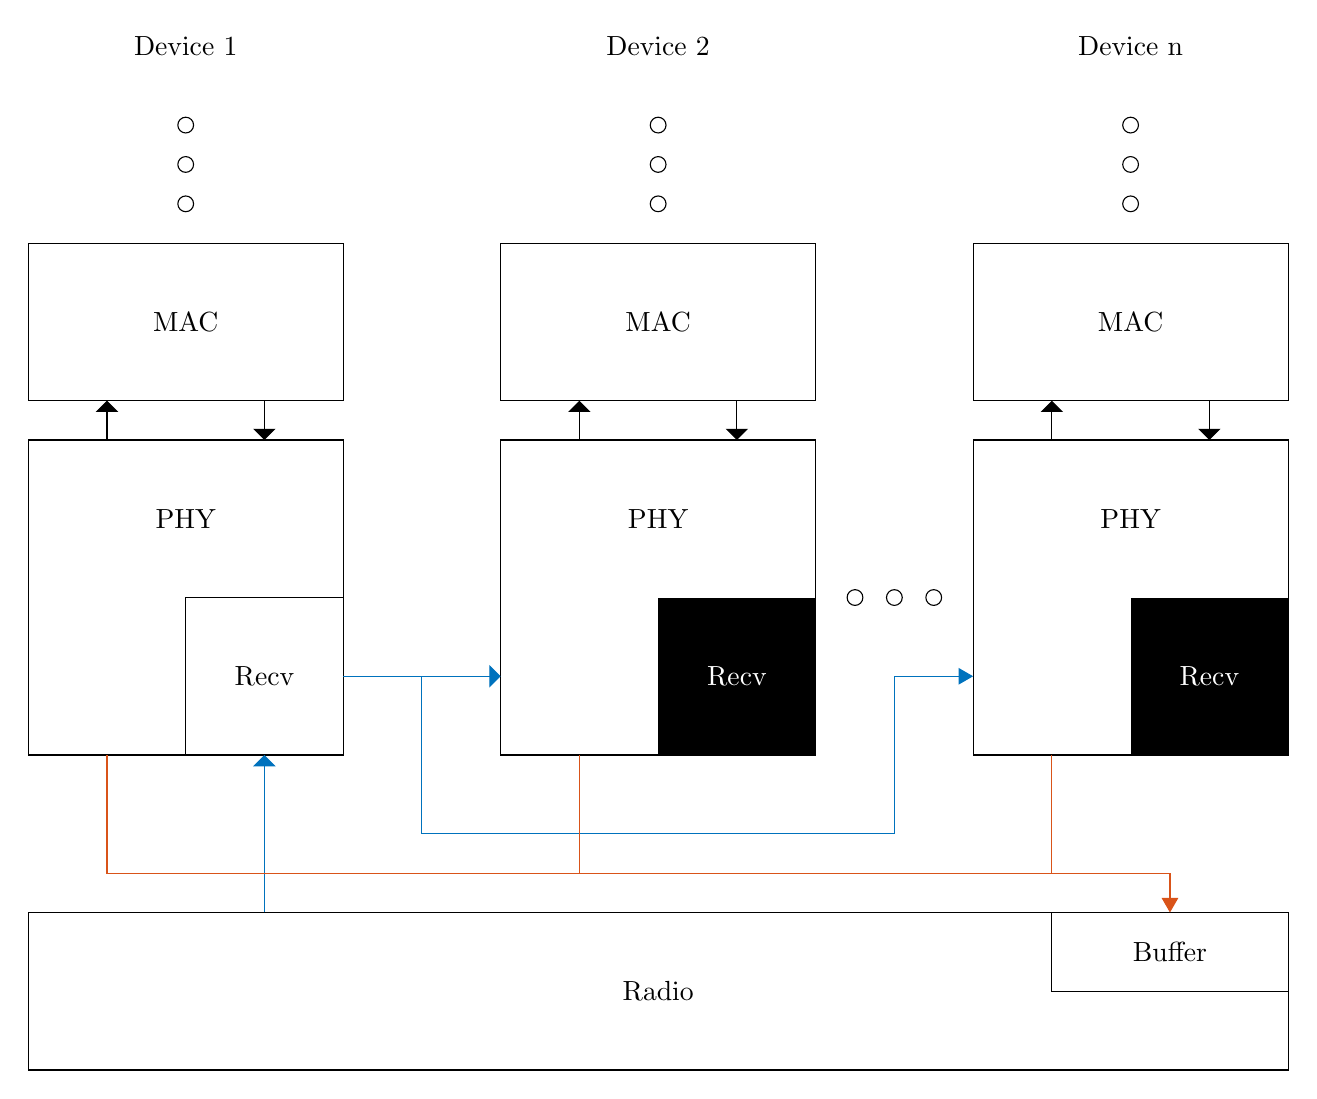
\begin{tikzpicture}

\draw  (-5,2.5) rectangle (-1,-1.5);
\draw  (-5,3) rectangle (-1,5);
\draw  (-3,-1.5) rectangle (-1,0.5);
\draw  (1,2.5) rectangle (5,-1.5);
\draw  (1,3) rectangle (5,5);
\fill [black](3,-1.5) rectangle (5,0.5);
\draw  (-3,6) ellipse (0.1 and 0.1);
\draw  (-3,5.5) ellipse (0.1 and 0.1);
\draw  (-3,6.5) ellipse (0.1 and 0.1);
\draw  (3,6) ellipse (0.1 and 0.1);
\draw  (3,5.5) ellipse (0.1 and 0.1);
\draw  (3,6.5) ellipse (0.1 and 0.1);
\draw  (5.5,0.5) ellipse (0.1 and 0.1);
\draw  (6,0.5) ellipse (0.1 and 0.1);
\draw  (6.5,0.5) ellipse (0.1 and 0.1);
\draw  (7,2.5) rectangle (11,-1.5);
\fill [black]  (9,-1.5) rectangle (11,0.5);
\draw  (7,3) rectangle (11,5);
\draw  (9,6) ellipse (0.1 and 0.1);
\draw  (9,5.5) ellipse (0.1 and 0.1);
\draw  (9,6.5) ellipse (0.1 and 0.1);
\node at (-3,7.5) {Device 1};
\node at (3,7.5) {Device 2};
\node at (9,7.5) {Device n};
\node at (-3,4) {MAC};
\node at (3,4) {MAC};
\node at (9,4) {MAC};
\node at (-3,1.5) {PHY};
\node at (3,1.5) {PHY};
\node at (9,1.5) {PHY};
\node at (-2,-0.5) {Recv};
\node [white]at (4,-0.5) {Recv};
\node [white]at (10,-0.5) {Recv};
\draw  (-5,-3.5) rectangle (11,-5.5);
\node at (3,-4.5) {Radio};
\draw  (8,-3.5) rectangle (11,-4.5);
\node at (9.5,-4) {Buffer};
\draw [-triangle 90](-4,2.5) -- (-4,3);
\draw [-triangle 90](-2,3) -- (-2,2.5);
\draw [-triangle 90](2,2.5) -- (2,3);
\draw [-triangle 90](4,3) -- (4,2.5);
\draw [-triangle 90](8,2.5) -- (8,3);
\draw [-triangle 90](10,3) -- (10,2.5);
\draw [-triangle 90][mycolor1](-2,-3.5) -- (-2,-1.5);
\draw [-triangle 90][mycolor1](-1,-0.5) -- (1,-0.5);
\draw [-triangle 60][mycolor1](0,-0.5) -- (0,-2.5) -- (6,-2.5) -- (6,-0.5) -- (7,-0.5);
\draw [-triangle 60][mycolor2](-4,-1.5) -- (-4,-3) -- (9.5,-3) -- (9.5,-3.5);
\draw [mycolor2](2,-1.5) -- (2,-3);
\draw [mycolor2](8,-1.5) -- (8,-3);
\end{tikzpicture}